\usetikzlibrary{arrows.meta}
\usetikzlibrary{shapes.geometric}

\tikzset{%
  >={Latex[width=4mm,length=4mm]},
  % Specifications for style of nodes:
            base/.style = {rectangle, rounded corners, draw=black,
                           minimum width=4cm, minimum height=1cm,
                           text centered, font=\sffamily},
  activityStarts/.style = {base, fill=blue!30},
       startstop/.style = {base, fill=red!30},
    activityRuns/.style = {base, fill=green!30},
         process/.style = {base, minimum width=2.5cm, fill=blue!15,
                           font=\sffamily},
         ifstatement/.style = {base, diamond, aspect=2.4},
}
% Drawing part, node distance is 1.5 cm and every node
% iss prefilled with white background

\begin{figure}
\centering
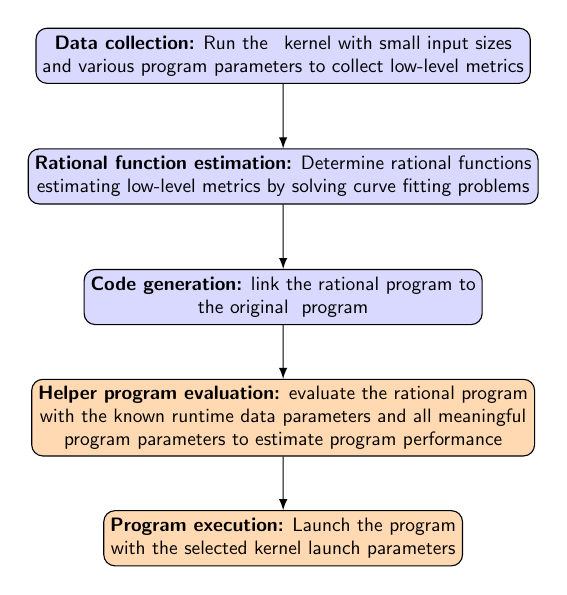
\begin{tikzpicture}[node distance=5cm,
every node/.style={fill=white, font=\sffamily, scale=0.7}, align=center]
% Specification of nodes (position, etc.)
\node (collection)             [process]              {\textbf{Data collection:} Run the \cuda\, kernel with small input sizes\\ and various program parameters to collect low-level metrics};
\node (curvefitting)     [process, below of=collection, yshift=8em]          {\textbf{Rational function estimation:} Determine rational functions\\ estimating low-level metrics by solving curve fitting problems};
%\node (ifmetric) [ifstatement, below of=curvefitting, yshift=-5em] {\small{Metrics without}\\ \small{Rational Functions?}};
%\node (dofit) [process, right of=ifmetric, xshift=20em] {Estimate Parameters of\\ Rational Function};
%\node (encoderatfun) [process, above of=dofit, yshift=0.5em] {Compute Rational Function\\ For Low-Level Metric};
\node (codegen)      [process, below of=curvefitting,yshift=8em]   {\textbf{Code generation:} link the rational program to\\ the original {\cuda} program};
\node (rateval)     [process,fill=orange!30, below of=codegen, yshift=8em]   {\textbf{Helper program evaluation:} evaluate the rational program\\ with the known runtime data parameters and all meaningful\\ program parameters to estimate program performance};
\node (execute)      [process,fill=orange!30, below of=rateval, yshift=8em] {\textbf{Program execution:} Launch the program \\with the selected kernel launch parameters};
\draw[-latex]             (collection) -- (curvefitting);
\draw[-latex]     (curvefitting) -- (codegen);
\draw[-latex]      (codegen) -- (rateval);
\draw[-latex]     (rateval) -- (execute);
\end{tikzpicture}
%\caption{Generating the rational program ${\cal R}$  when compiling 
%the multithreaded program ${\cal P}$
%then using  ${\cal R}$ to optimize the execution of ${\cal P}$. }
\label{fig:sixsteps}
\end{figure}
